\documentclass[12pt]{article}
\usepackage[margin=1in]{geometry}
\usepackage{setspace}
\usepackage{amsmath}
\usepackage{array}
\usepackage{float}
\usepackage{graphicx}
\usepackage{caption}
\usepackage{hyperref}
\usepackage{mathptmx}

\doublespacing
\setlength{\parindent}{0.5in}
\setlength{\parskip}{0pt}
\pagestyle{plain}
\urlstyle{same}

\newcommand{\aparef}[1]{\par\noindent\hangindent=0.5in\hangafter=1 #1\par}

\begin{document}

\begin{titlepage}
\thispagestyle{empty}
\begin{center}
\vspace*{1.75in}
{\Large A Knowledge-Graph Contagion Mapping Framework for Systemic Risk in India's Credit Sector\par}
\vspace{1.5in}
{[Author Name]\par}
\vspace{0.25in}
{[Department], [Institution Name]\par}
\vspace{0.25in}
{[Course Code: Course Name]\par}
\vspace{0.25in}
{[Instructor Name]\par}
\vspace{0.25in}
{April 10, 2026\par}
\end{center}
\end{titlepage}

\section*{Abstract}

The 2018 default of Infrastructure Leasing \& Financial Services Limited (IL\&FS) exposed how little visibility Indian market participants had into layered credit dependencies, related-party exposures, and subsidiary structures. This paper develops a knowledge-graph framework for mapping contagion risk in the Indian credit sector using public and market-facing disclosures. The proposed system integrates CRISIL lender-facility data, Ministry of Corporate Affairs master data, NSE shareholding and filing disclosures, Reserve Bank of India supervisory tables, Basel III Pillar 3 reports, and FinBERT-based news sentiment. From CRISIL's FY2024-25 rated universe of 9,911 entities, the framework retains 2,858 entities with exposures above INR 50 crore, representing approximately 29\% of the rated universe and INR 36.73 lakh crore in systemically relevant exposure. Stress is modeled as a bounded node score and propagated across lending, ownership, subsidiary, related-party, and industry edges through fixed-point iteration. The resulting network is sparse at the system level but highly concentrated around a small number of hubs and bridge institutions. These findings support the argument that systemic vulnerability in India cannot be assessed from entity-level balance sheets alone. The framework offers a practical foundation for early warning, scenario analysis, and risk surveillance for regulators, banks, and institutional investors.

\noindent\textit{Keywords:} systemic risk, knowledge graph, financial contagion, India, credit networks

\newpage
\begin{center}
\textbf{A Knowledge-Graph Contagion Mapping Framework for Systemic Risk in India's Credit Sector}
\end{center}

\section*{Introduction}
September 2018. Infrastructure Leasing & Financial Services Limited (IL&FS)—a shadow lender rated investment-grade by three agencies—defaulted on ₹1,000 Crore commercial paper (Ministry of Corporate Affairs, 2018). Within weeks, investigators discovered the group held ₹91,000 Crores debt distributed across 348 subsidiaries, built on parent equity of just ₹9.83 Crores (Serious Fraud Investigation Office, 2019). A debt-to-equity ratio of 9,257:1.

The contagion was swift. Over 300 NBFC and Housing Finance Company stocks lost between 20-70% value in the following quarter (NSE India, 2018). Mutual funds holding IL&FS paper faced redemption pressures; DSP Mutual Fund's forced sale of DHFL commercial paper triggered its own spiral. Credit spreads for AAA-rated NBFCs widened 100 basis points overnight (RBI Financial Stability Report, December 2018). The banking regulator, then-RBI Governor Urjit Patel, compared it to India's own "Lehman moment" (Reuters, 2018). Government intervened by superseding the IL&FS board—an unprecedented step under Companies Act 2013.

What made this crisis uniquely instructive was not the fraud alone, but the blindness. 179 of IL&FS's 348 subsidiaries had never been reported in consolidated financial statements (Grant Thornton Forensic Audit, 2019). Credit rating agencies maintained "AAA" and "AA+" ratings months before default. RBI's own Financial Stability Reports from 2017-2018 made no mention of IL&FS risk. The pipes connecting India's financial system—short-term borrowings refinanced daily, inter-corporate deposits, related-party guarantees—were invisible until they burst.

This paper introduces a Knowledge Graph-based framework for mapping these hidden connections before they fracture.

We construct a unified network of 2,858 entities from CRISIL's FY2024-25 rated universe of 9,911 entities—representing approximately 29% by entity count but capturing the systemically significant exposures above ₹50 Crores (totaling ₹36.73 lakh crore). The framework integrates CRISIL credit ratings, MCA filings for subsidiary and related-party transaction data, Basel III Pillar 3 disclosures, and real-time news sentiment via FinBERT. It provides infrastructure for contagion scenario analysis: tracing how hypothetical defaults propagate through second and third-order network connections.

Three constituencies stand to benefit. For regulators—RBI, SEBI—it offers an early warning layer complementing entity-level supervision. For bank risk teams calculating Expected Credit Loss under Ind AS 109, network maps reveal counterparty exposures that internal models currently miss. For institutional investors, stress scores provide independent signals where rating agency assessments have demonstrably lagged.

\section*{Literature Review}

Financial contagion operates like an epidemic. Allen and Gale (2000) first formalized this intuition: liquidity withdrawal at one bank cascades through networks, with transmission speed depending on topology—not individual institution health. Their insight launched two decades of systemic risk measurement.

Acharya et al. (2017) introduced Marginal Expected Shortfall (MES), measuring institutional loss during market-wide downturns. Brownlees and Engle (2017), including a Nobel laureate, extended this to SRISK—capital shortfall conditional on prolonged market decline. Both approaches, now used by CAFRAL and IIMs for Indian bank assessment, share one limitation: they require market prices, excluding India's substantial unlisted corporate and NBFC universe.

Network-based approaches address this gap. Battiston et al. (2012) developed DebtRank, propagating stress through exposure-weighted edges; Adrian and Brunnermeier (2016) contributed ΔCoVaR for institution-level systemic contribution. The IMF's SyRIN framework (2018) operationalized these concepts for emerging markets. Caccioli et al. (2020) demonstrated that financial networks exhibit "robust-yet-fragile" properties—absorbing small-node failures while remaining vulnerable when hubs collapse. This finding underpins our threshold-based entity filtering.

Indian credit market literature has grown rapidly. Bajaj and Damodaran (2023) identified Domestic Systemically Important Banks using component expected shortfall, documenting increasing NBFC contribution to aggregate network risk. Dash et al. (2023) mapped Indian bank interconnections using ΔCoVaR, distinguishing "good links" (liquidity sharing) from "bad links" (contagion channels). Poddar et al. (2023) employed Panel VAR to visualize bank interconnectedness during downturns. The RBI's Financial Stability Reports acknowledge concentration risk: default by top three borrowers would raise system GNPA by 350 basis points (RBI, 2025).

For real-time signals, FinBERT (Araci, 2019) enables domain-specific sentiment analysis, capturing financial meanings—"restructuring," "NPA," "covenant breach"—that generic models miss. Stander (2024) constructed a FinBERT-based news sentiment index demonstrating causal relationship with systemic risk indicators, directly validating sentiment as a leading indicator for IFRS 9/Ind AS 109 impairment modeling.

Knowledge graphs have recently entered financial risk literature. Chen and Zhang (2023) applied KG embeddings to study liquidity-to-systemic risk transmission in banking networks, published in *Journal of Financial Stability*. Their approach uses market-data-driven embeddings; ours differs by constructing the graph directly from regulatory filings and corporate relationship disclosures—capturing unlisted entities invisible to market-based methods.

**The Gap**: No existing framework unifies network mapping (lending, shareholding, subsidiary chains), real-time sentiment analysis, credit fundamentals, and contagion scenario analysis into operational infrastructure for Indian markets. Market-dependent measures cannot assess unlisted entities. Static network models lack forward-looking sentiment signals. Rating agencies lag actual distress by months. Entity-level supervision misses network amplification. This paper addresses all four limitations.

\section*{Research Motivation and Problem Statement}

### Why India, Why Now

India's banking sector has tripled in ten years—credit expanded from ₹66.91 lakh crore to ₹181.34 lakh crore (Press Information Bureau, 2025). NBFCs now account for roughly 25% of credit intermediation (RBI FSR, 2024). The IMF's 2025 FSAP praised this as making the system "more diverse and interconnected"—diversity reducing concentration, interconnectedness introducing new fragility (IMF, 2025).

Indian markets present unique research conditions. Unlike developed economies where bilateral exposure databases exist (Fed Y-14, ECB AnaCredit), Indian credit relationships must be inferred from regulatory disclosures. Unlike markets dominated by listed entities, Indian corporates include substantial unlisted exposure requiring non-market-based stress assessment. IL&FS provided a natural experiment validating network-based concerns.

### The Information Asymmetry Problem

Picture a bank credit committee evaluating a corporate borrower. They possess: financial statements, credit rating, sector outlook. They do not observe: the borrower's full subsidiary structure, real-time sentiment shifts signaling governance concerns, other creditors' stress levels, or second-order exposures through the borrower's own loan book.

RBI does maintain CRILC—Central Repository of Information on Large Credits—mandating banks report all exposures ≥₹5 Crore (RBI Master Direction, 2014). But CRILC data stays siloed within regulatory systems. Banks cannot see other banks' CRILC data. Market participants operate blind to the full network. Hence asymmetry persists for everyone except the regulator—who lacks real-time sentiment integration.

\begin{enumerate}
\item Can a knowledge graph architecture effectively represent multi-layer relationships—lending, shareholding, subsidiary ownership, related-party transactions—characterizing Indian financial networks?
\item Does integrating FinBERT sentiment analysis with historical credit metrics improve early warning capability relative to credit ratings alone?
\item Can fixed-point contagion propagation, applied to constructed networks, trace stress patterns consistent with historical crises—specifically IL&FS 2018?
\end{enumerate}

## Scope

Our framework covers 41 Scheduled Commercial Banks, NBFCs including Housing Finance Companies, and primary corporate borrowers. We exclude: mutual fund portfolio holdings (data constraints), insurance interconnections (separate regulatory domain), OTC derivatives (bilateral data unavailable), cross-border linkages (complexity beyond present scope).

The entity universe comprises 2,858 entities with exposures exceeding ₹50 Crores, selected from CRISIL's FY2024-25 rated universe of 9,911 entities. This threshold—aligned with RBI's CRILC monitoring intensity—captures systemically significant exposures totaling ₹36.73 lakh crore while reducing network complexity for computational tractability. The filtering is theoretically grounded in Caccioli et al.'s (2020) finding that systemic risk concentrates in highly-connected hubs.

\section*{Method}

\subsection*{Data Sources}

The methodology begins from a practical constraint: systemic mapping in India must often be inferred from fragmented disclosures rather than downloaded from a single exposure registry. The framework addresses this problem by integrating five main layers of evidence: NSE shareholding and integrated filing disclosures, Ministry of Corporate Affairs master data, CRISIL lender-facility information, Reserve Bank of India statistical tables, and Basel III Pillar 3 disclosures (CRISIL Ratings, n.d.; NSE India, n.d.-a, n.d.-b; Open Government Data Platform India, n.d.; Reserve Bank of India, n.d.-a).

For banks, the extracted data include balance-sheet structure, supervisory ratios, outstanding advances to priority sectors, related-party disclosures, and shareholding pattern information. For companies, the primary fields include lender-facility relationships from rating reports, legal identity and industrial classification from Ministry of Corporate Affairs records, and ownership information from market disclosures. This combination is important because lender-facility data create direct credit edges, while corporate identity and ownership data make it possible to preserve subsidiary and dependency structures rather than collapsing entities into flat borrower lists.

Asset and Liability data was crucial for understanding the structure of a bank’s exposure. The initial idea was to identify how a company’s default would push the bank closer to a default using the distance to default metric. This idea stemmed from the Special Feature in ECB’s 2004 Financial Review, titled “Cross Border Bank Contagion”. The authors used weekly differenced distance to default to understand how contagion spread in Europe, and differentiate between a systemic shock and a contagion.

The balance-sheet mix differs across Indian bank groups. For the 41 Scheduled Commercial Banks in our consideration, which does not cover Foreign Banks, advances covered >60\% of their assets. This made it clear, that mapping these advances is critical to understand major portion of their exposure.

\begin{table}[h]
\centering
\begin{minipage}{\textwidth}
\textbf{Table 1}\\
\textit{Balance-Sheet Heterogeneity Across Bank Groups}
\end{minipage}
\vspace{0.1in}

\begin{tabular}{p{1.7in}cccc}
\hline
Bank Group & Advances (\% of Assets) & Investments (\% of Assets) & Deposits (\% of Liabilities) & Borrowings (\% of Liabilities) \\
\hline
Public sector banks & 62.71 & 24.90 & 82.82 & 6.91 \\
Private sector banks & 64.55 & 22.77 & 73.40 & 10.05 \\
Foreign banks & 30.21 & 45.17 & 54.01 & 16.45 \\
Small finance banks & 67.20 & 21.53 & 77.79 & 7.40 \\
\hline
\end{tabular}
\end{table}

The advances data came from CRISIL Reports of companies where they had to disclose their Bank Facilities, which mention the amount of loan and lender name. In total, data of 9919 companies were gathered. Around ~97\%ile of total loan amount(from the CRISIL Data) was captured by 2848 companies. However, this does not map all advances of the selected 41 banks. Due to limitations of data available, only ~10\% of their advances have been mapped.

\subsection*{Stress Modeling}

Stress is modeled as a bounded score in the interval from 0 to 1, where higher values indicate greater fragility. The model is designed to be interpretable rather than purely black-box. The general idea is to use bank ratios to calculate the stress on a bank using Principal Component Analysis, or rather Kernel PCA which is a non-linear version of PCA. This stress score is blended with other components including news stress that is calculated using the FinBERT model. 

Raw supervisory ratios are transformed into health scores using direction-aware rules anchored to the Reserve Bank of India's Prompt Corrective Action thresholds for capital adequacy and asset quality (Reserve Bank of India, n.d.-b). Those transformed features are then embedded through the RBF kernel that captures non-linear dependence across capital, liquidity, profitability, and asset quality dimensions. The bank score is blended with a Merton-style distance-to-default orientation, a CAMELS-style supervisory composite, and news stress. When all components are available, the implementation uses the following weighted blend:

\[
\text{Bank stress} = 0.23 B_d + 0.23 B_c + 0.27 B_m + 0.27 N
\]

where $B_d$ is the boundary-distance signal, $B_c$ is the CAMELS-style composite, $B_m$ is the Merton-oriented component, and $N$ is news stress.

For companies, stress is decomposed into three components: fundamental credit stress, news stress, and sector stress. Fundamental stress is derived from the rating and lender-facility structure, including downgrade risk, concentration, staleness, exposure size, and coverage gaps. The node-level company score is assembled adaptively according to data availability:

\[
\text{Company stress} =
\begin{cases}
0.7E + 0.2N + 0.1S, & \text{if } E, N, S \text{ are available} \\
0.8E + 0.2N, & \text{if sector stress is missing} \\
0.8E + 0.2S, & \text{if news stress is missing} \\
E, & \text{if only fundamental stress is available}
\end{cases}
\]

where $E$ is fundamental stress, $N$ is news stress, and $S$ is sector stress.

The news pipeline uses recent articles and filing text snippets, scores them with FinBERT, and converts sentiment into a stress signal (Araci, 2019). At the snippet level, the transformation is:

\[
\text{Snippet stress} = P(\text{negative}) + 0.5 P(\text{neutral})
\]

This design ensures that a strongly negative article immediately raises local stress even before the next rating review or annual filing update.

\subsection*{Knowledge Graph Construction and Contagion Propagation}

The graph is directed and weighted. Banks, companies, and industries form the main node types. The most important relationship families are \texttt{LENDS\_TO}, \texttt{SHAREHOLDER\_OF}, \texttt{RELATED\_PARTY}, \texttt{SUBSIDIARY\_OF}, and \texttt{BELONGS\_TO}. The graph therefore captures both direct loss channels and slower-moving dependence channels such as ownership and related-party concentration.

A central design choice is to preserve unresolved entities as explicit stubs rather than dropping them. This matters because missing counterparties are often exactly where hidden contagion pathways begin. If a lender or related party cannot be fully resolved, the framework still creates a placeholder node so that the path structure remains visible and auditable.

Stress propagation is implemented as a synchronous fixed-point process. Let $s_i^{(0)}$ denote the baseline stress of node $i$, and let $w_{ji}$ denote the transmission weight on the edge from node $j$ to node $i$. Incoming stress in round $t$ is:

\[
I_i^{(t)} = \sum_{j:(j \to i)} s_j^{(t-1)} w_{ji}
\]

The updated node stress is then:

\[
s_i^{(t)} = \min \left(1, \max \left(0, s_i^{(0)} + I_i^{(t)} \right)\right)
\]

Iterations continue until the maximum change across nodes falls below a small tolerance threshold or a fixed iteration limit is reached. This approach is simple, transparent, and well suited to scenario analysis because it re-anchors every round on baseline fragility while still allowing the network to amplify stress.

\subsection*{Technical Architecture}

The implementation separates storage, graph persistence, and visualization. MongoDB acts as the operational source of truth for normalized bank, company, and sector documents. Neo4j materializes the graph for traversal, subgraph extraction, and simulation. This division allows extraction and feature engineering to evolve without constantly redefining graph persistence logic.

Entity resolution is managed through a Global Entity Registry. The resolver uses canonical exact matching first, normalized exact matching second, constrained fuzzy matching for companies third, and bank-specific abbreviation handling last. Bank resolution is deliberately conservative so that similarly named affiliates are not accidentally merged into parent institutions.

On top of the database layer, a React and Three.js visualizer provides a bank-centered exploration interface. The visualizer is not just cosmetic. It supports neighborhood discovery, path tracing, and topology inspection, which makes the framework more useful for analysts conducting targeted stress investigations.

\section*{Results}

The model reveals a highly concentrated but economically interpretable connectivity structure across banks, NBFCs, and large corporate borrowers. The network is sparse at full-system level (density = 0.000145) but contains a small set of hubs and bridge entities that dominate path-based contagion reach.

\subsection*{1. Bank Connectivity Pattern}

\begin{figure}[H]
\centering
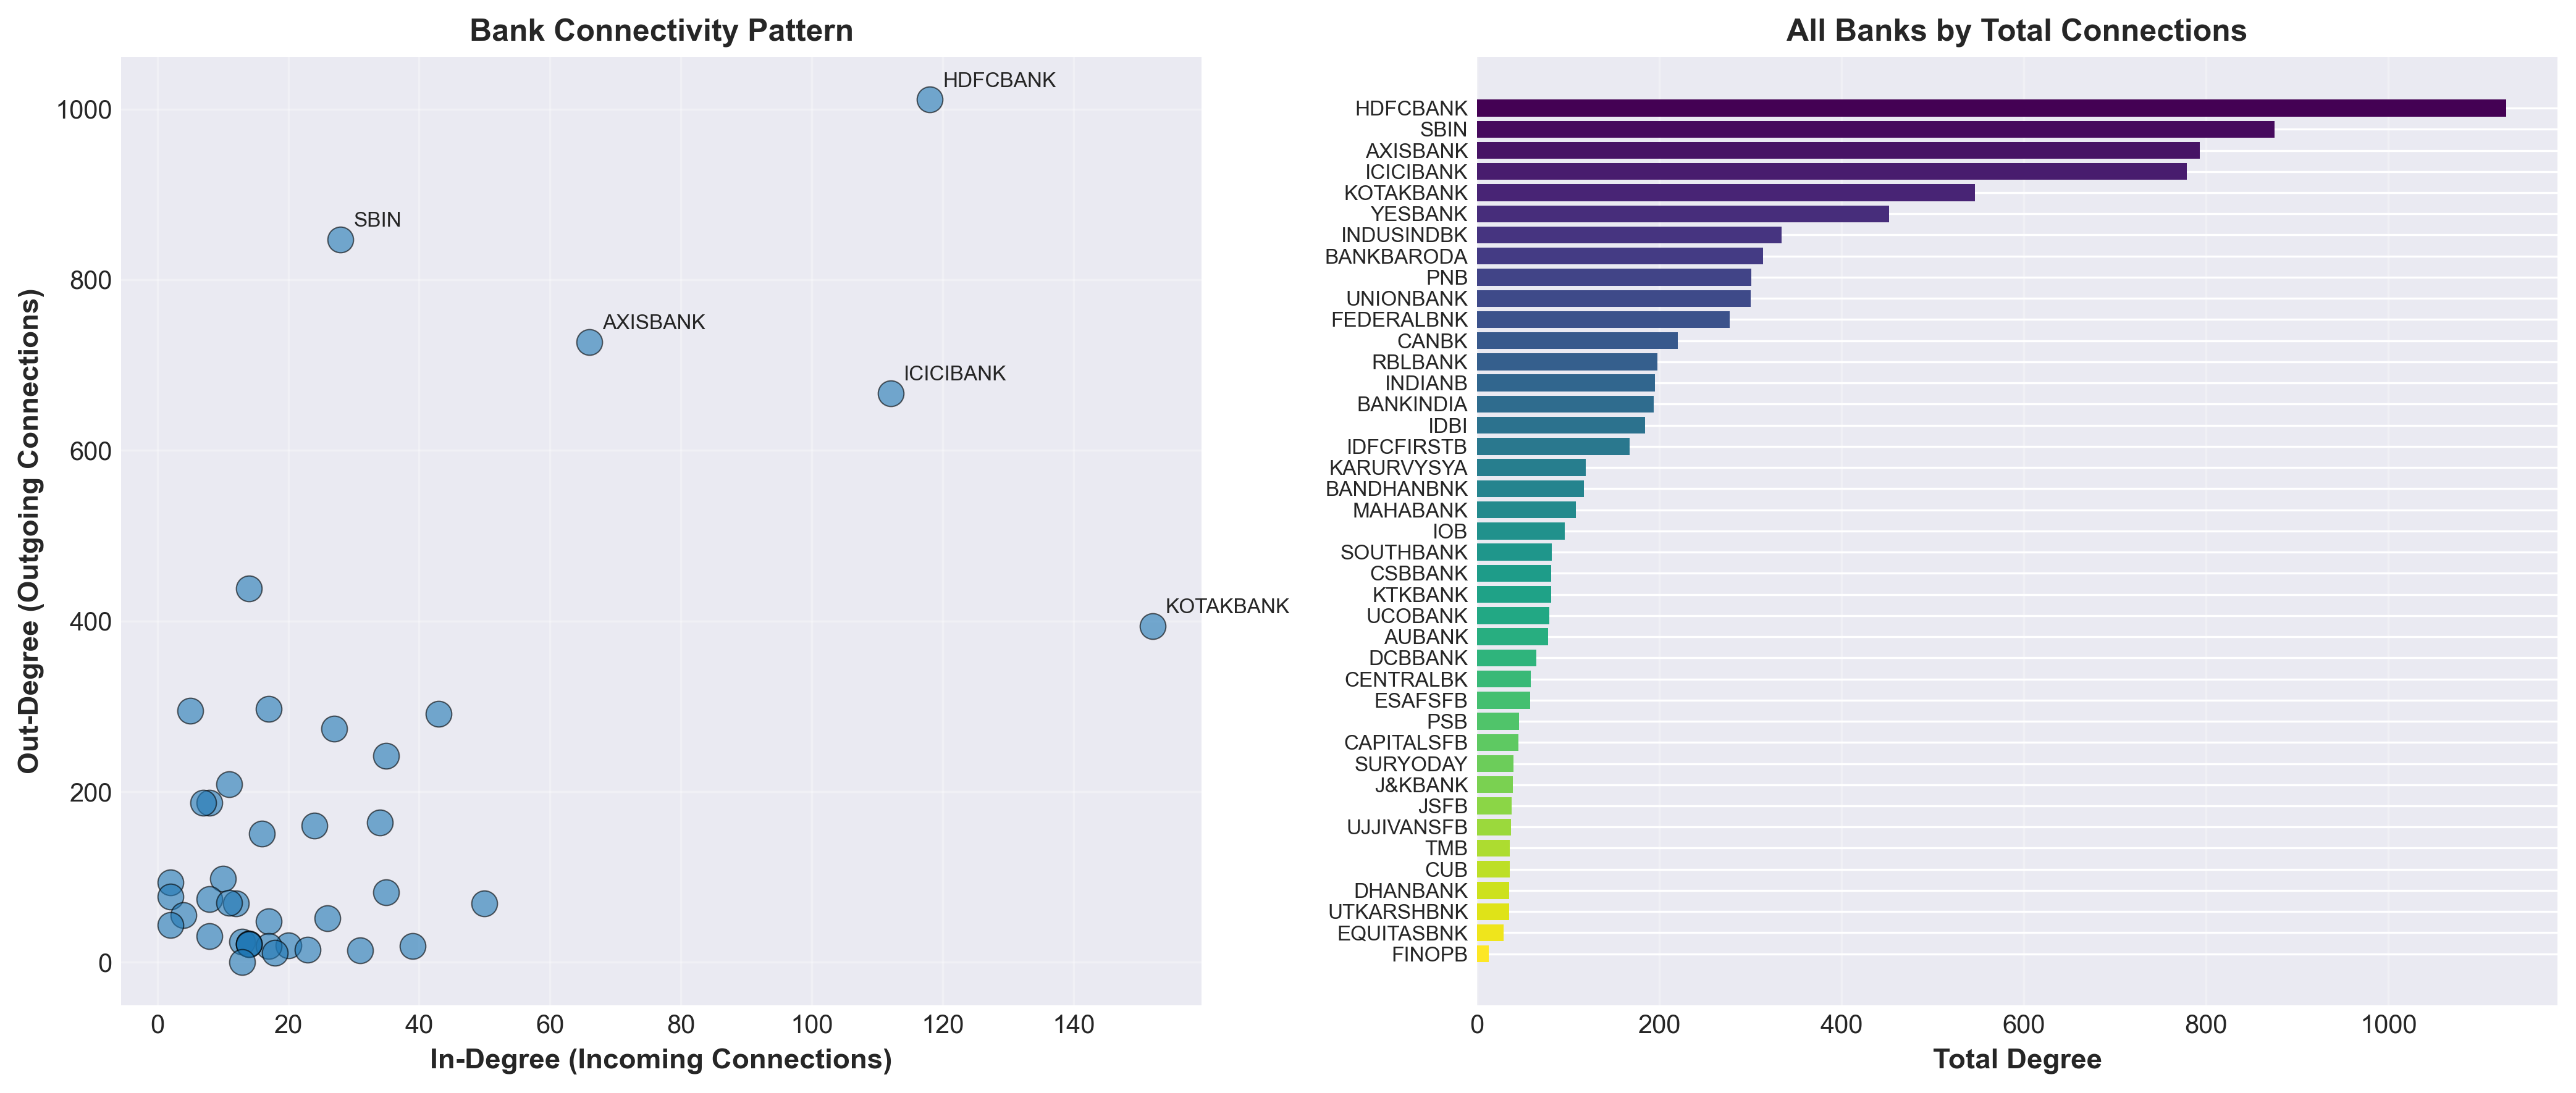
\includegraphics[width=\textwidth]{./figures/fig6_bank_degree_distribution.png}
\caption*{Figure 6. Bank connectivity pattern and total degree ranking}
\end{figure}

The degree structure is strongly skewed. A small set of banks account for a disproportionately large share of total graph connectivity, while the long tail has low degree and limited systemic reach.

\begin{table}[H]
\centering
\small
\begin{tabular}{l l r r r}
\hline
Rank (Total Degree) & Bank & In-Degree & Out-Degree & Total Degree \\
\hline
1 & HDFCBANK & 118 & 1,011 & 1,129 \\
2 & SBIN & 28 & 847 & 875 \\
3 & AXISBANK & 66 & 727 & 793 \\
4 & ICICIBANK & 112 & 667 & 779 \\
5 & KOTAKBANK & 152 & 394 & 546 \\
\hline
\end{tabular}
\end{table}

HDFCBANK and SBIN behave as broad connectivity hubs (very high out-degree), while KOTAKBANK exhibits the highest in-degree, indicating stronger concentration of incoming links into that node. This suggests distinct systemic roles: large outward transmission capacity for some banks, versus high incoming dependency concentration for others.

\subsection*{2. Largest Corporate Exposure Concentrations}

\begin{figure}[H]
\centering
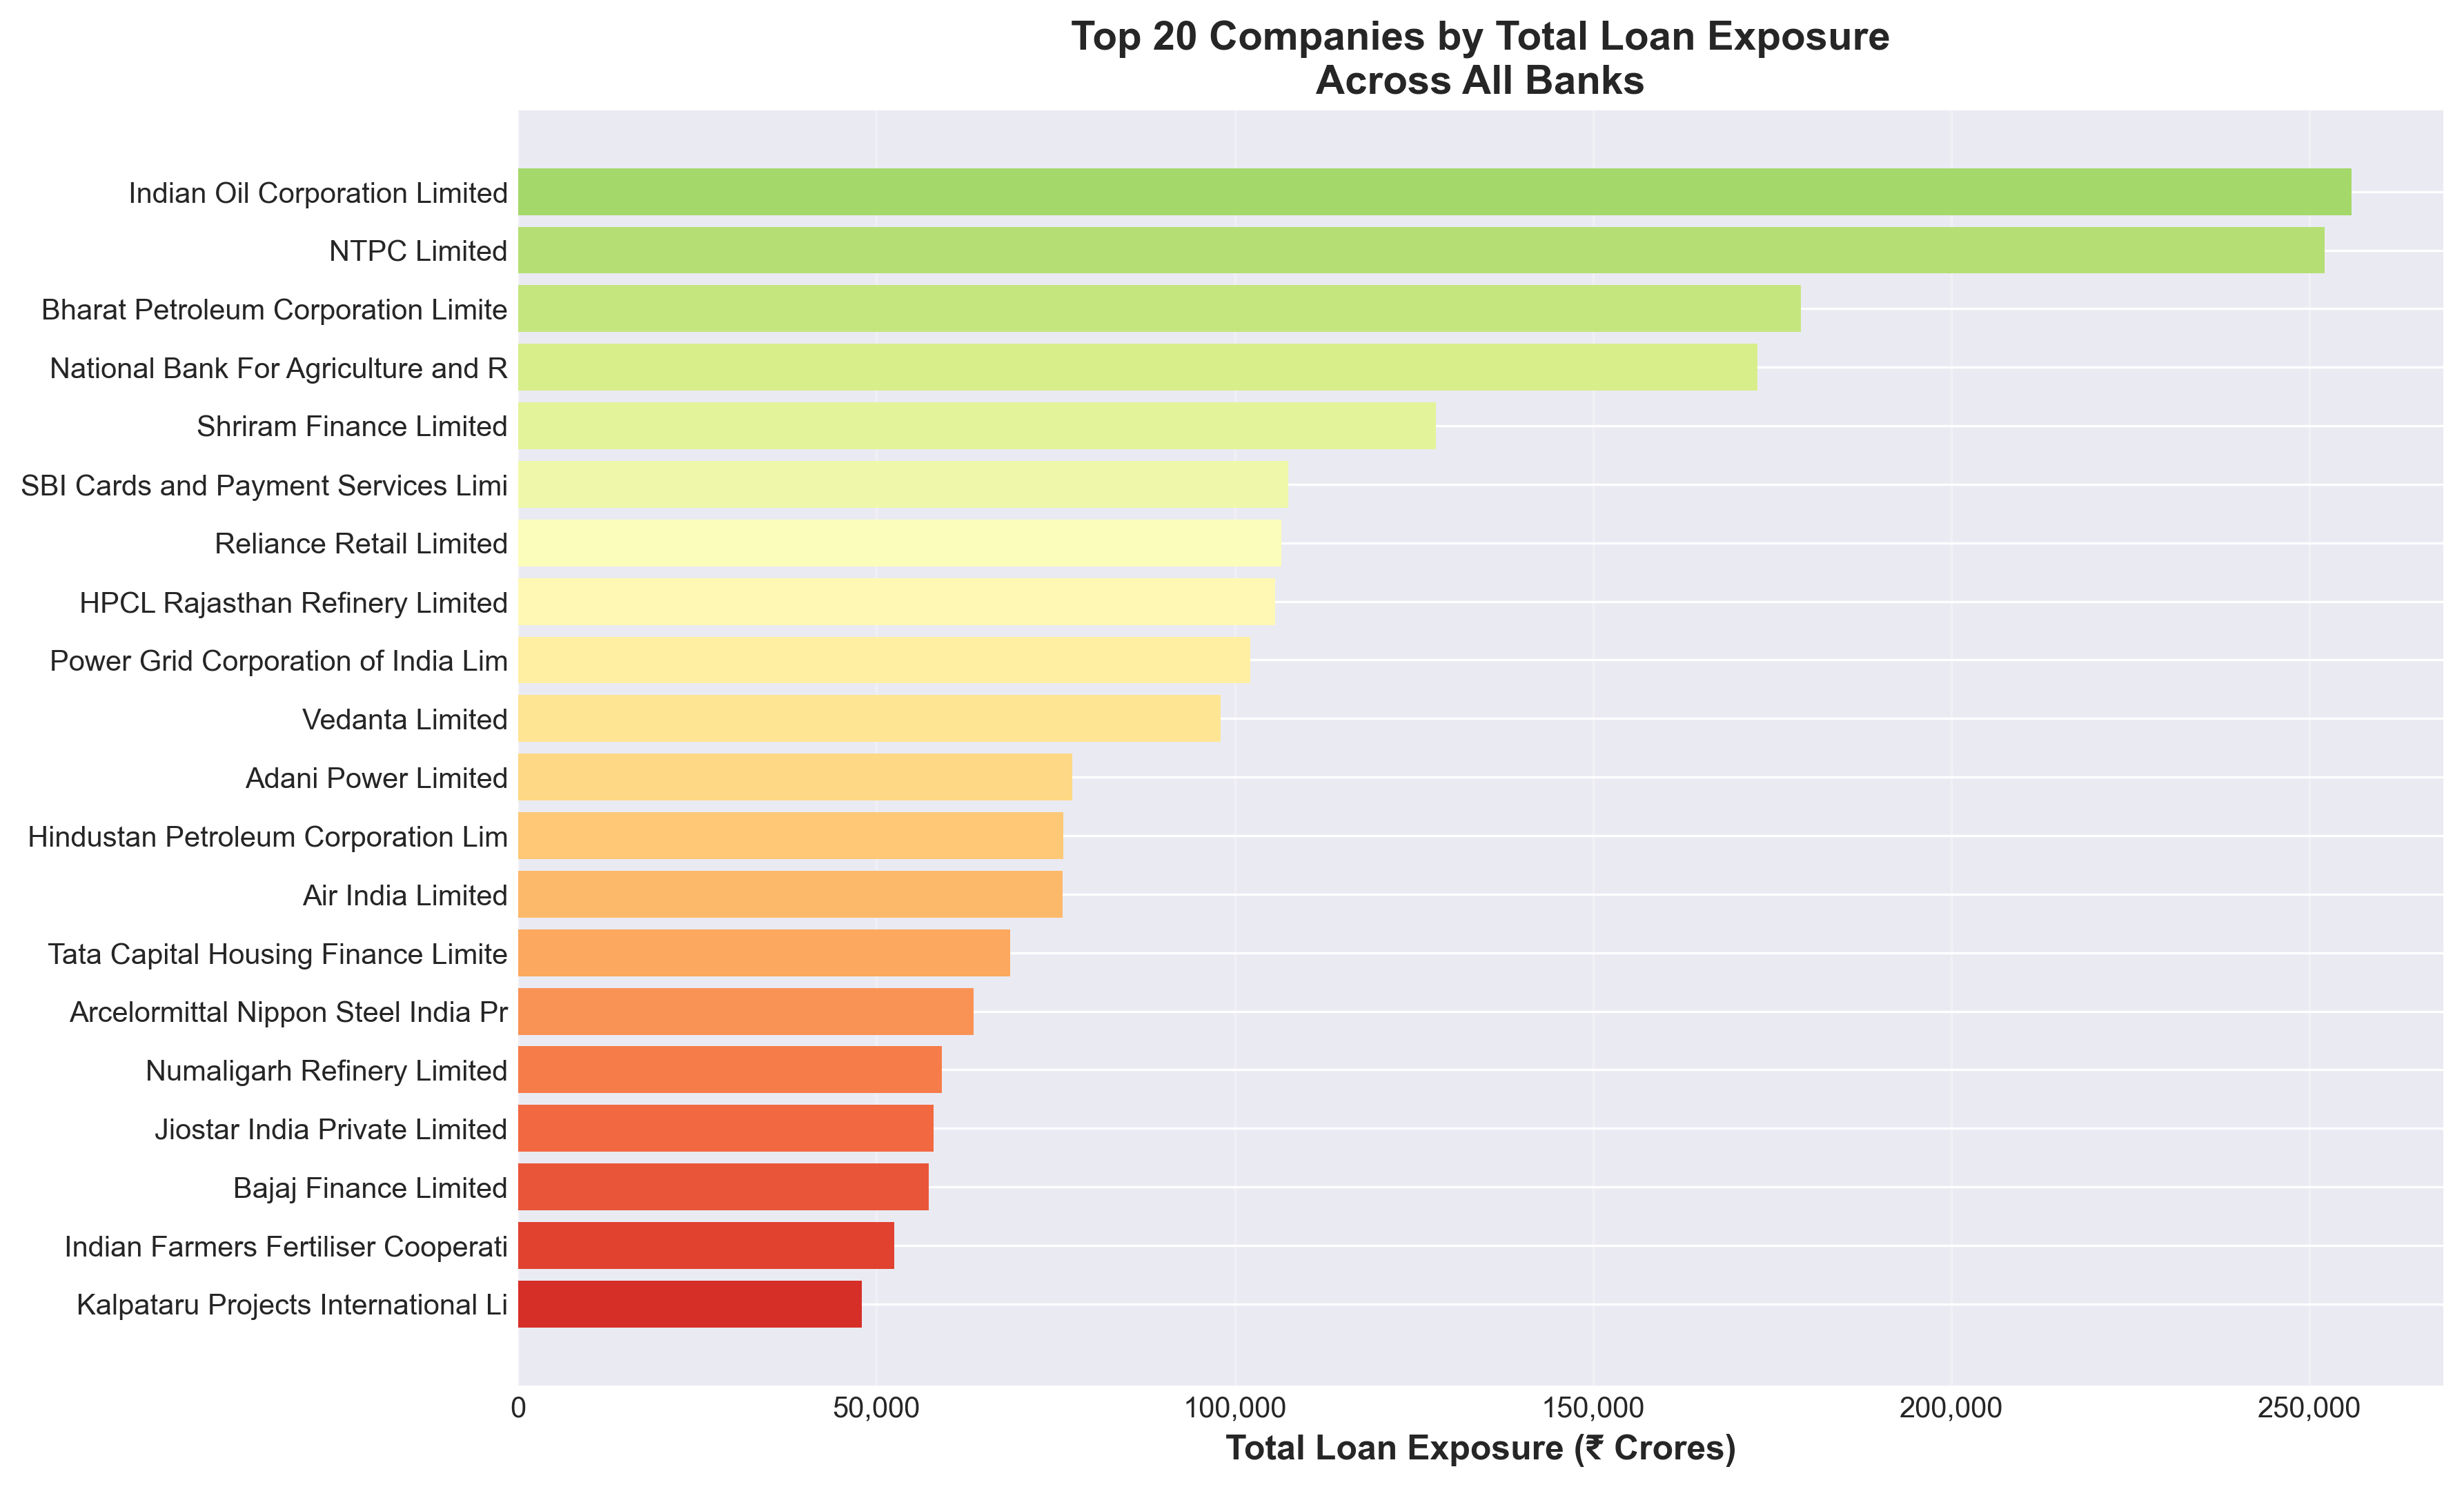
\includegraphics[width=\textwidth]{./figures/fig7_top_companies_by_exposure.png}
\caption*{Figure 7. Top companies by total loan exposure}
\end{figure}

The largest observed exposures are concentrated in a limited subset of large borrowers (oil and gas, power, and financial intermediaries), with a visible drop after the top 3--5 names.

\begin{table}[H]
\centering
\small
\begin{tabular}{r p{3.4in} r r}
\hline
Rank & Company & Total Loan Exposure (INR Cr) & Number of Lenders \\
\hline
1 & Indian Oil Corporation Limited & 255,866.00 & 16 \\
2 & NTPC Limited & 252,068.64 & 19 \\
3 & Bharat Petroleum Corporation Limited & 178,993.06 & 19 \\
4 & National Bank for Agriculture and Rural Development & 172,933.10 & 8 \\
5 & Shriram Finance Limited & 128,023.28 & 55 \\
\hline
\end{tabular}
\end{table}

Note: These exposure rankings come from the observed lender-facility layer in the integrated snapshot. Only 100 companies in the extracted exposure table carry the required loan-edge structure, against 3,497 company nodes in the full graph (about 2.86\%). Therefore, this should be interpreted as a high-confidence but partial view of the full corporate credit universe.

\subsection*{3. Centrality and Systemic Positioning}

\begin{figure}[H]
\centering
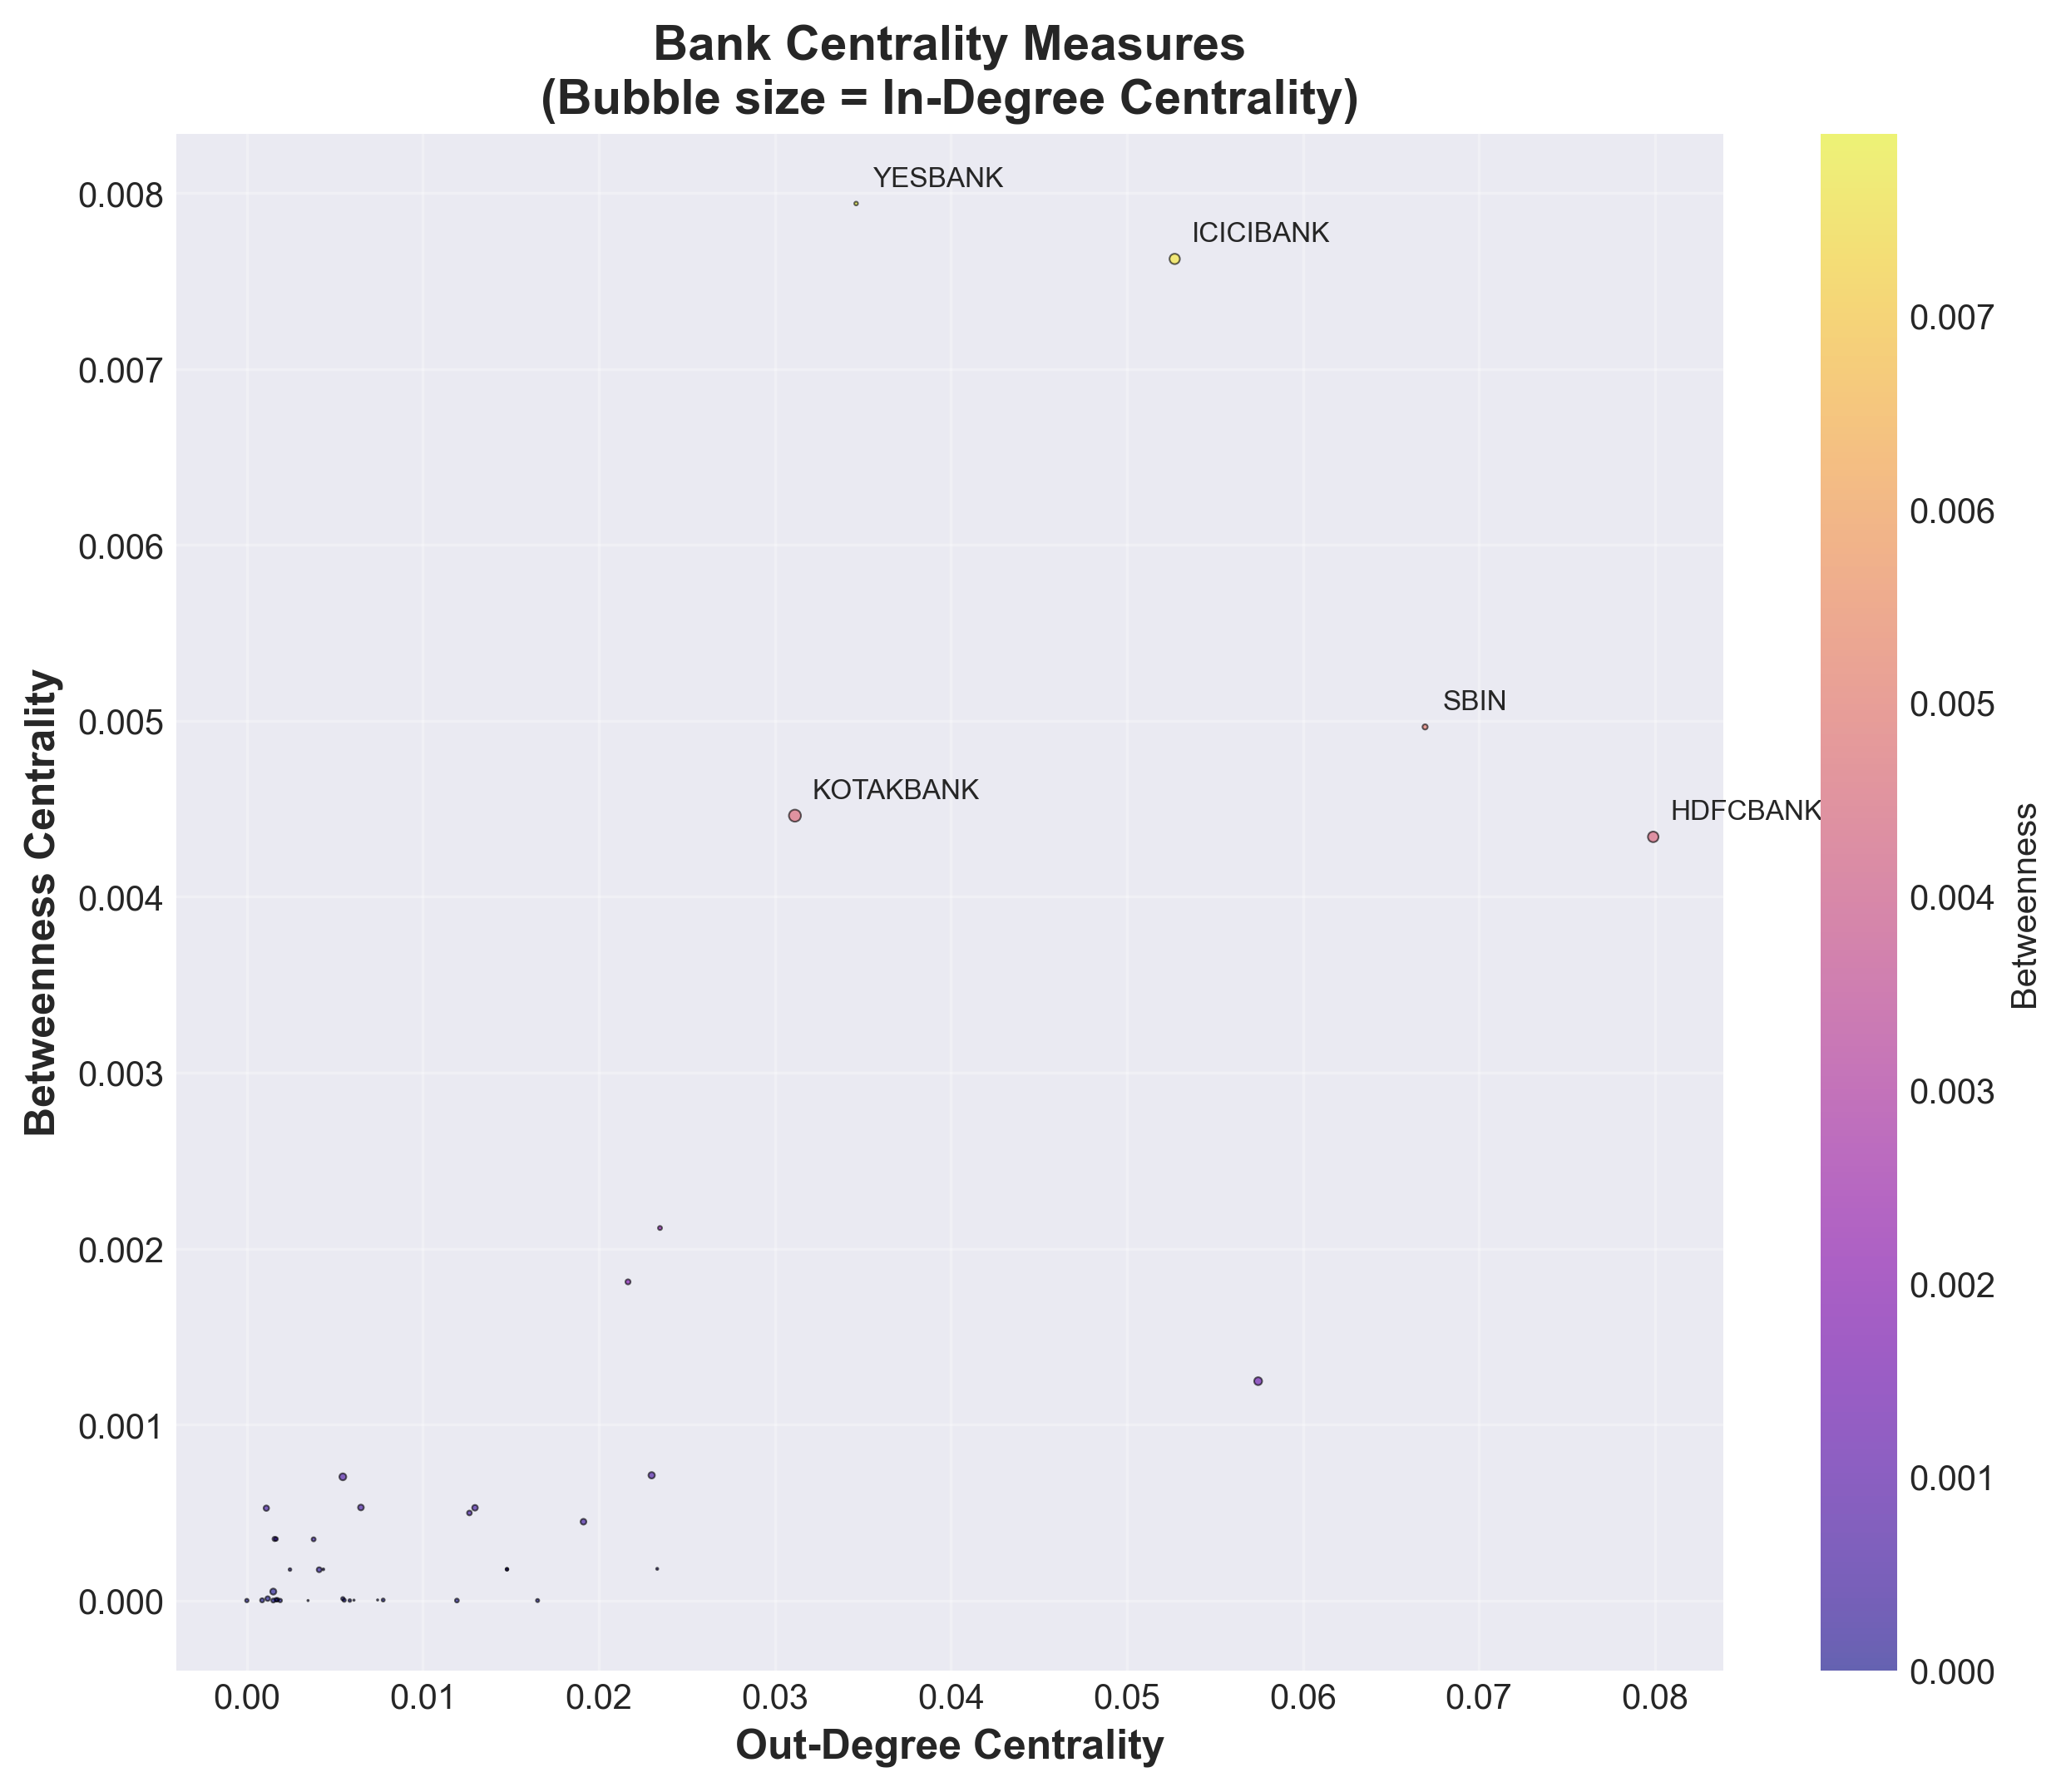
\includegraphics[width=\textwidth]{./figures/fig9_bank_centrality_comparison.png}
\caption*{Figure 9. Bank centrality comparison}
\end{figure}

Centrality results separate ``highly connected'' from ``structurally pivotal.'' In particular, betweenness highlights bridging importance even when raw degree is not maximal.

\begin{table}[H]
\centering
\small
\begin{tabular}{l l r r r}
\hline
Rank (Betweenness) & Bank & Betweenness & Out-Degree Centrality & In-Degree Centrality \\
\hline
1 & YESBANK & 0.00794 & 0.03462 & 0.00111 \\
2 & ICICIBANK & 0.00763 & 0.05271 & 0.00885 \\
3 & SBIN & 0.00497 & 0.06694 & 0.00221 \\
4 & KOTAKBANK & 0.00446 & 0.03114 & 0.01201 \\
5 & HDFCBANK & 0.00434 & 0.07990 & 0.00933 \\
\hline
\end{tabular}
\end{table}

YESBANK emerges as the top bridge by betweenness despite much lower total degree than HDFCBANK and SBIN. Managerially, this indicates that degree-led surveillance alone can miss critical routing nodes where shocks can traverse between otherwise separate network regions.

\subsection*{4. Structural Bridge Nodes (Non-Bank Intermediaries)}

\begin{figure}[H]
\centering
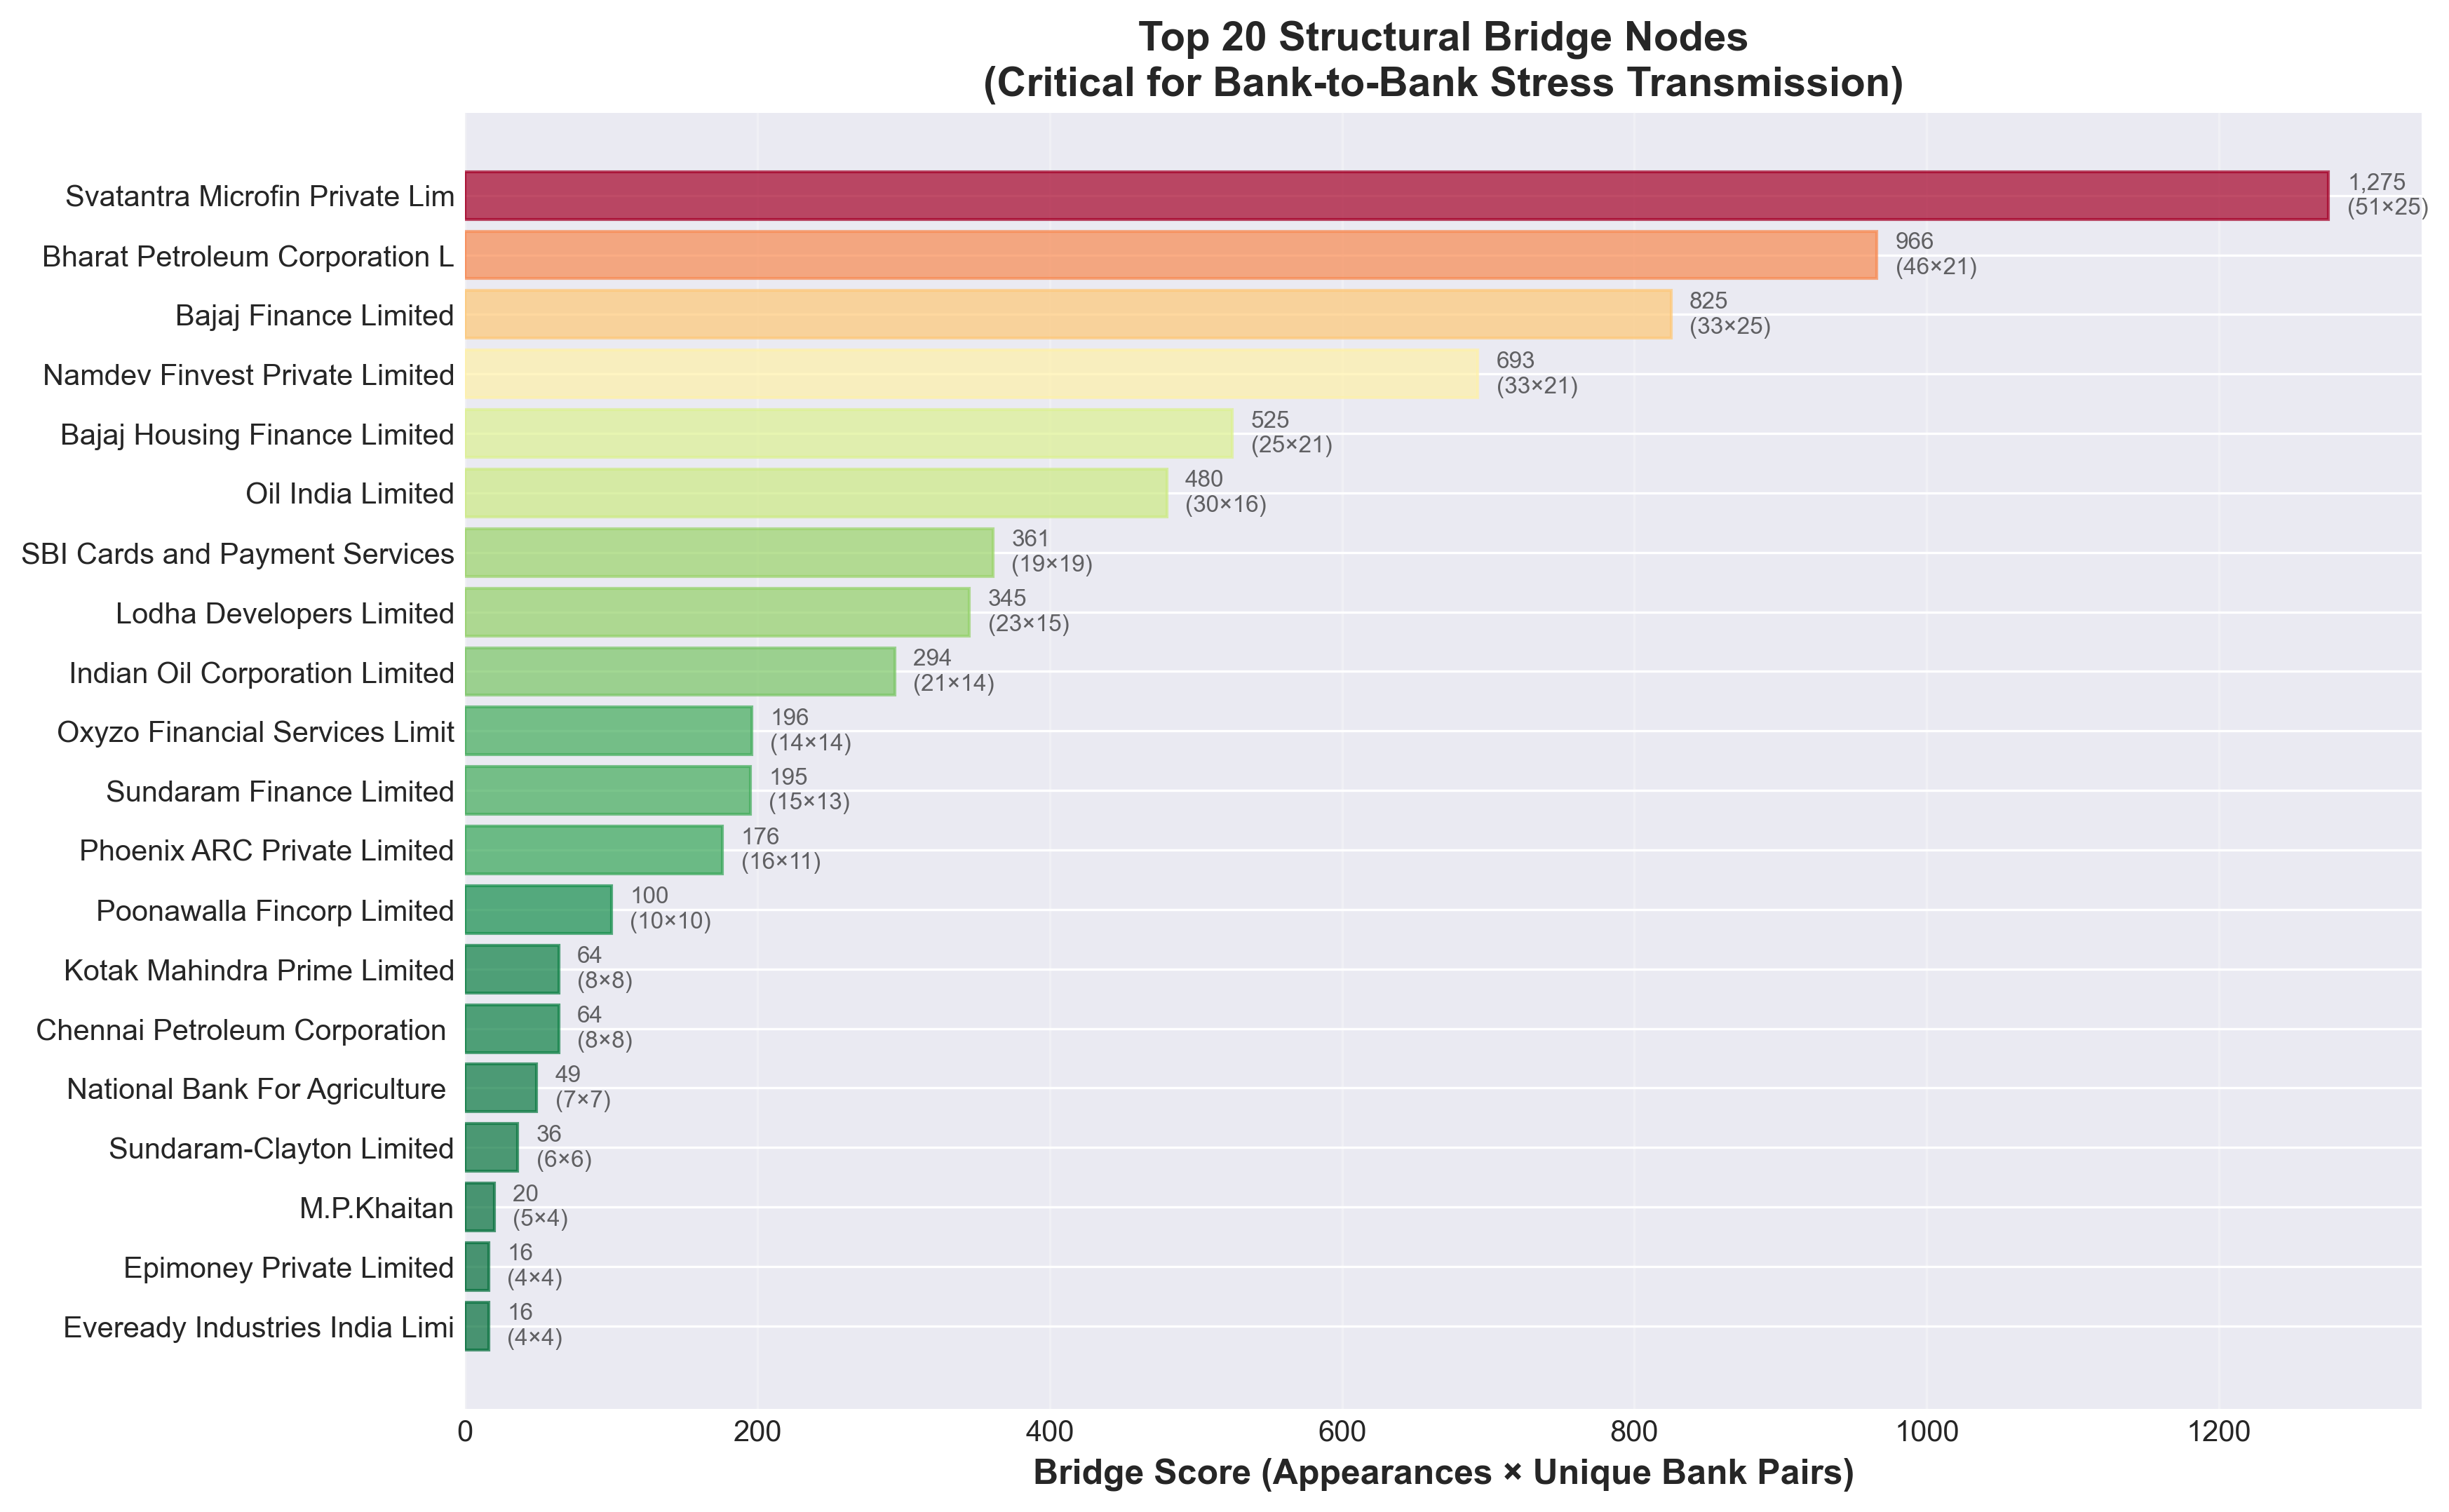
\includegraphics[width=\textwidth]{./figures/fig11_bridge_node_importance.png}
\caption*{Figure 11. Structural bridge node importance}
\end{figure}

Bridge-node analysis confirms that non-bank intermediaries are central to bank-to-bank contagion pathways. The bridge score is defined as:

\[
\mathrm{Bridge\ Score} = \mathrm{Path\ Appearances} \times \mathrm{Unique\ Bank\ Pairs}
\]

\begin{table}[H]
\centering
\small
\begin{tabular}{r p{2.8in} r r r}
\hline
Rank & Node & Path Appearances & Unique Bank Pairs & Bridge Score \\
\hline
1 & Svatantra Microfin Private Limited & 51 & 25 & 1,275 \\
2 & Bharat Petroleum Corporation Limited & 46 & 21 & 966 \\
3 & Bajaj Finance Limited & 33 & 25 & 825 \\
4 & Namdev Finvest Private Limited & 33 & 21 & 693 \\
5 & Bajaj Housing Finance Limited & 25 & 21 & 525 \\
\hline
\end{tabular}
\end{table}

Interpretation: contagion routing is not purely bank-to-bank; it is materially mediated by high-connectivity NBFCs and large operating corporates. This reinforces the need for cross-entity supervision rather than bank-only network diagnostics.

\subsection*{5. Bank-to-Bank Connectivity Paths}

\begin{figure}[H]
\centering
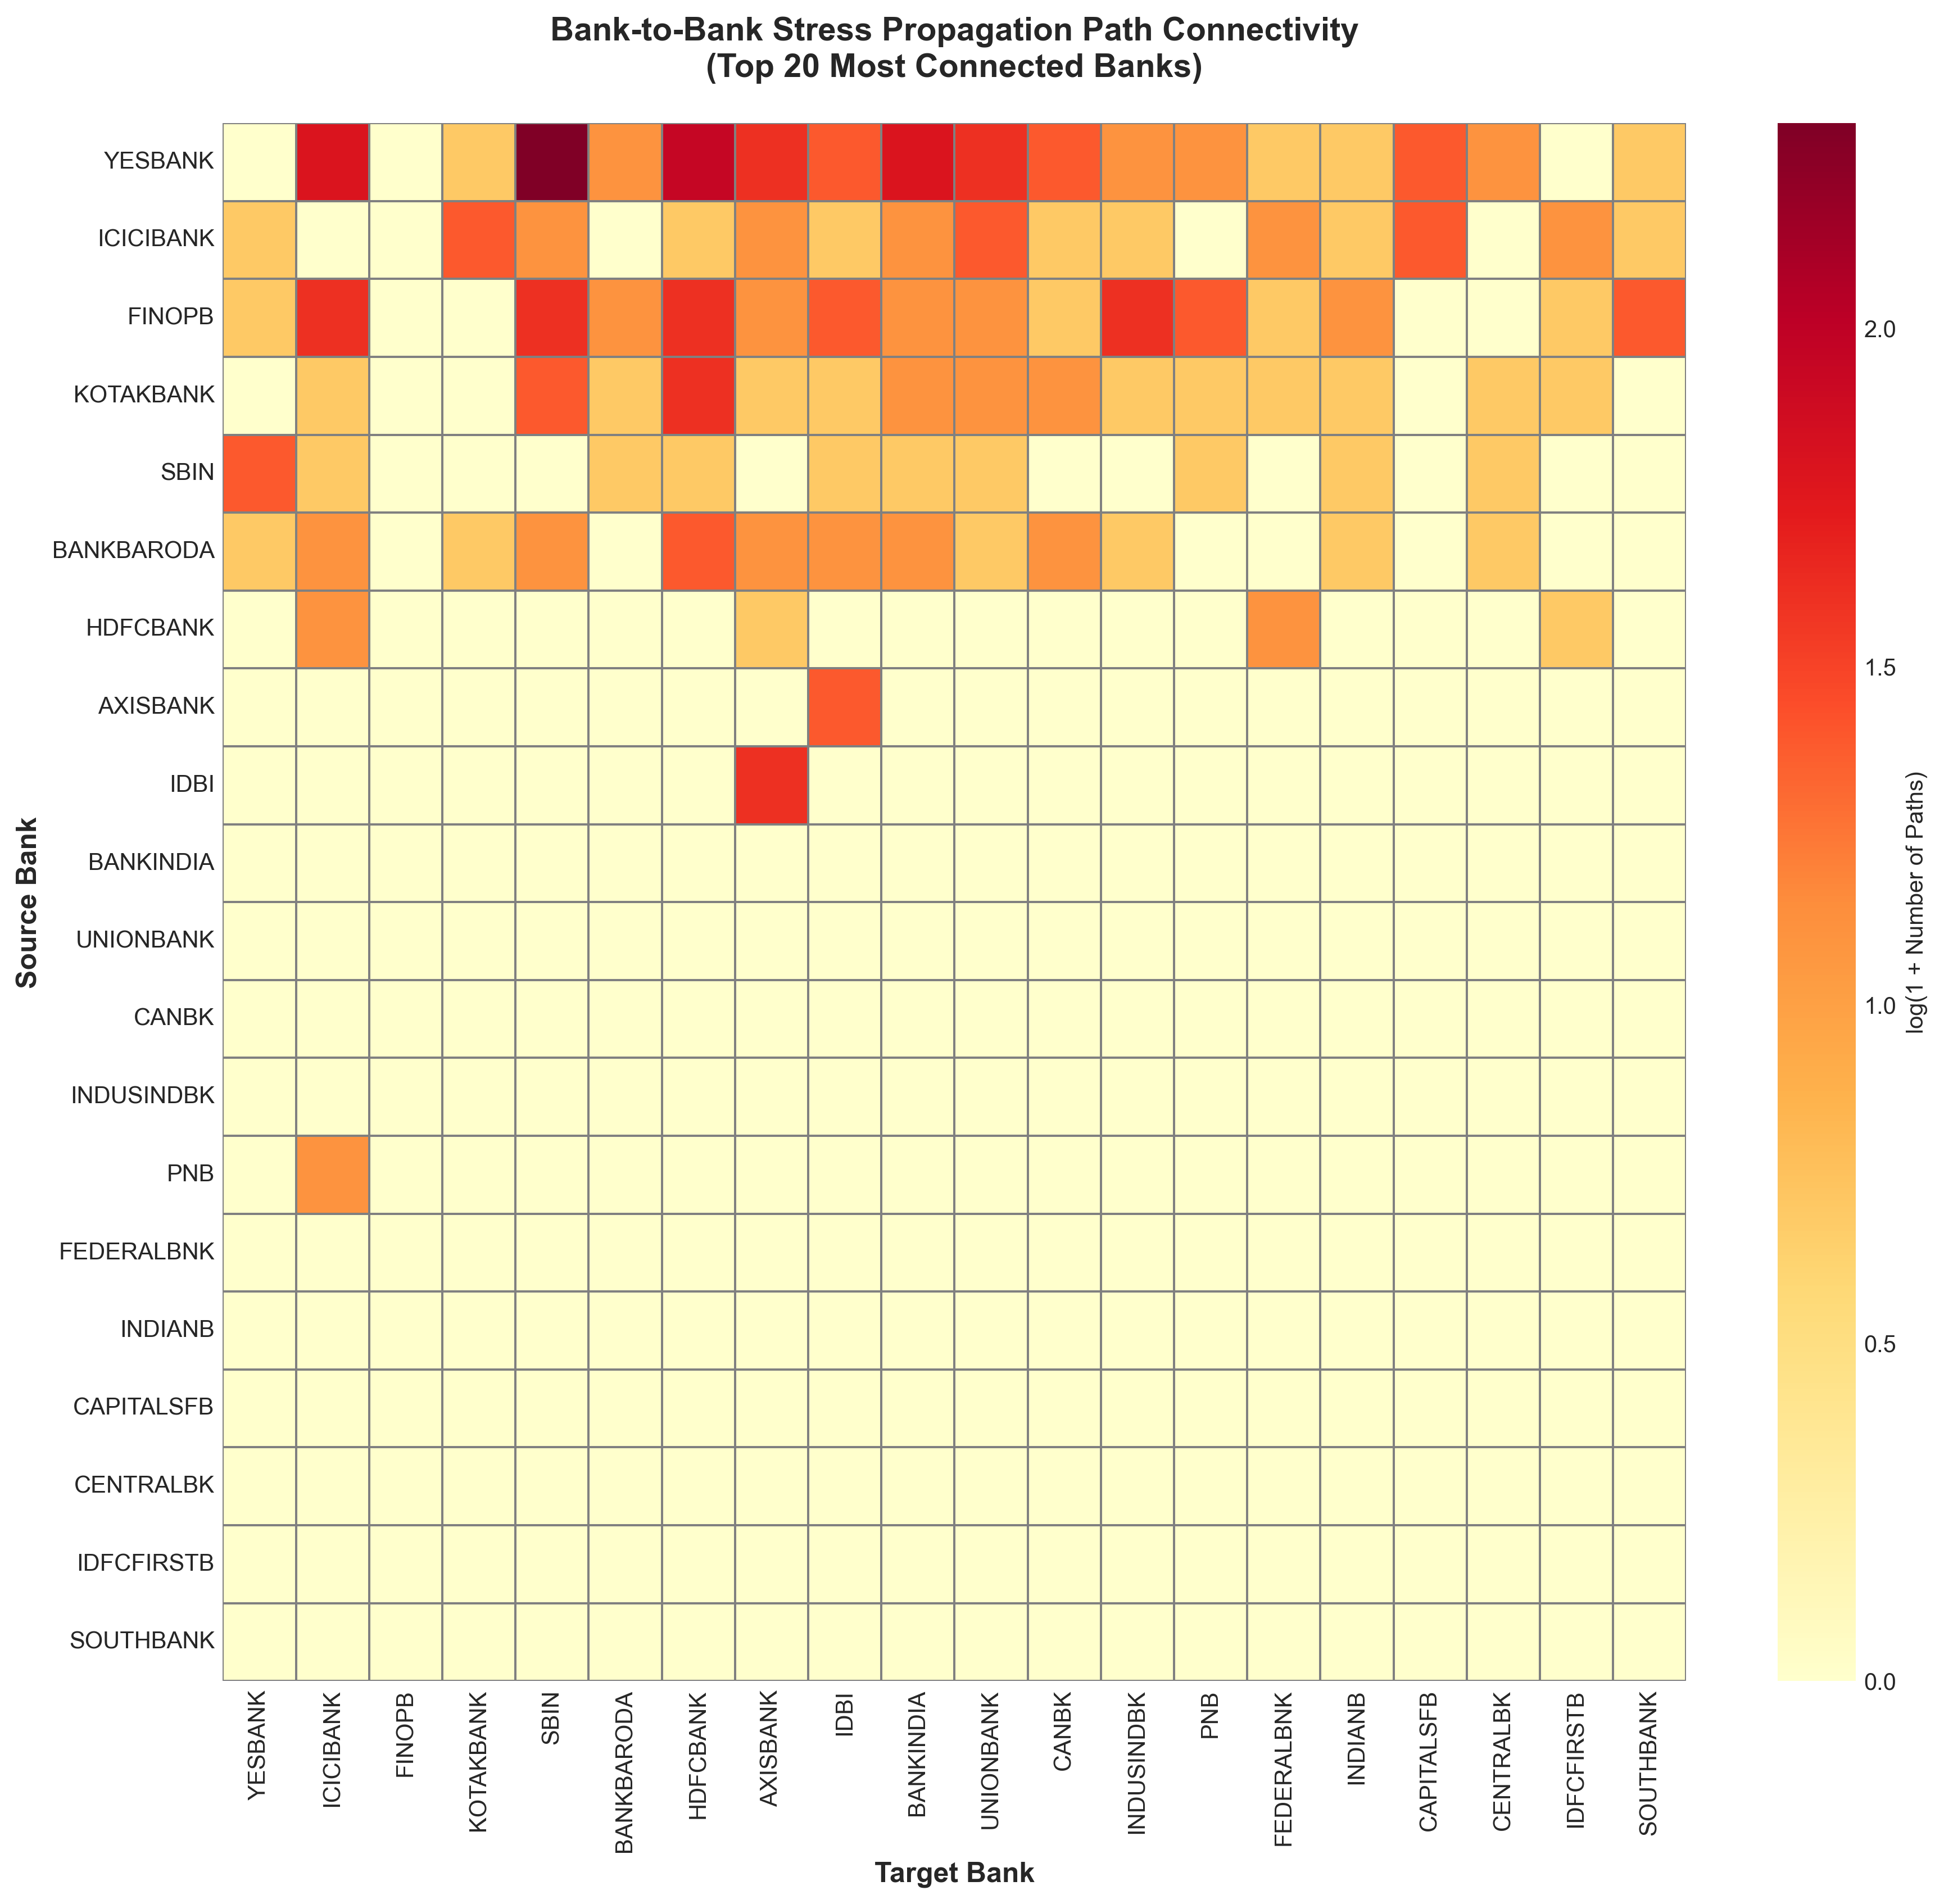
\includegraphics[width=\textwidth]{./figures/fig12_bank_connectivity_matrix.png}
\caption*{Figure 12. Bank-to-bank path connectivity matrix}
\end{figure}

The connectivity matrix highlights directional asymmetry in path multiplicity. Some banks generate many more outward reachable path combinations than others.

\begin{table}[H]
\centering
\small
\begin{tabular}{l l r r}
\hline
Rank (Source Connectivity) & Source Bank & Total Paths Across Pairs & Number of Reachable Bank Pairs \\
\hline
1 & YESBANK & 63 & 26 \\
2 & FINOPB & 46 & 21 \\
3 & ICICIBANK & 35 & 22 \\
4 & KOTAKBANK & 28 & 20 \\
5 & BANKBARODA & 23 & 15 \\
\hline
\end{tabular}
\end{table}

\begin{table}[H]
\centering
\small
\begin{tabular}{p{2.8in} r r r}
\hline
Most Connected Pair (Examples) & Number of Paths & Shortest Hops & Longest Hops \\
\hline
YESBANK $\to$ SBIN & 9 & 1 & 4 \\
YESBANK $\to$ HDFCBANK & 6 & 2 & 4 \\
YESBANK $\to$ ICICIBANK & 5 & 2 & 4 \\
YESBANK $\to$ BANKINDIA & 5 & 2 & 4 \\
FINOPB $\to$ SBIN & 4 & 2 & 5 \\
\hline
\end{tabular}
\end{table}

a few source banks account for most of the multi-path contagion reach. The YESBANK row concentration in the heatmap and the path table together indicate high routing optionality from this node to multiple large banks.

\subsection*{6. Shortest and Longest Path Structure}

\begin{figure}[H]
\centering
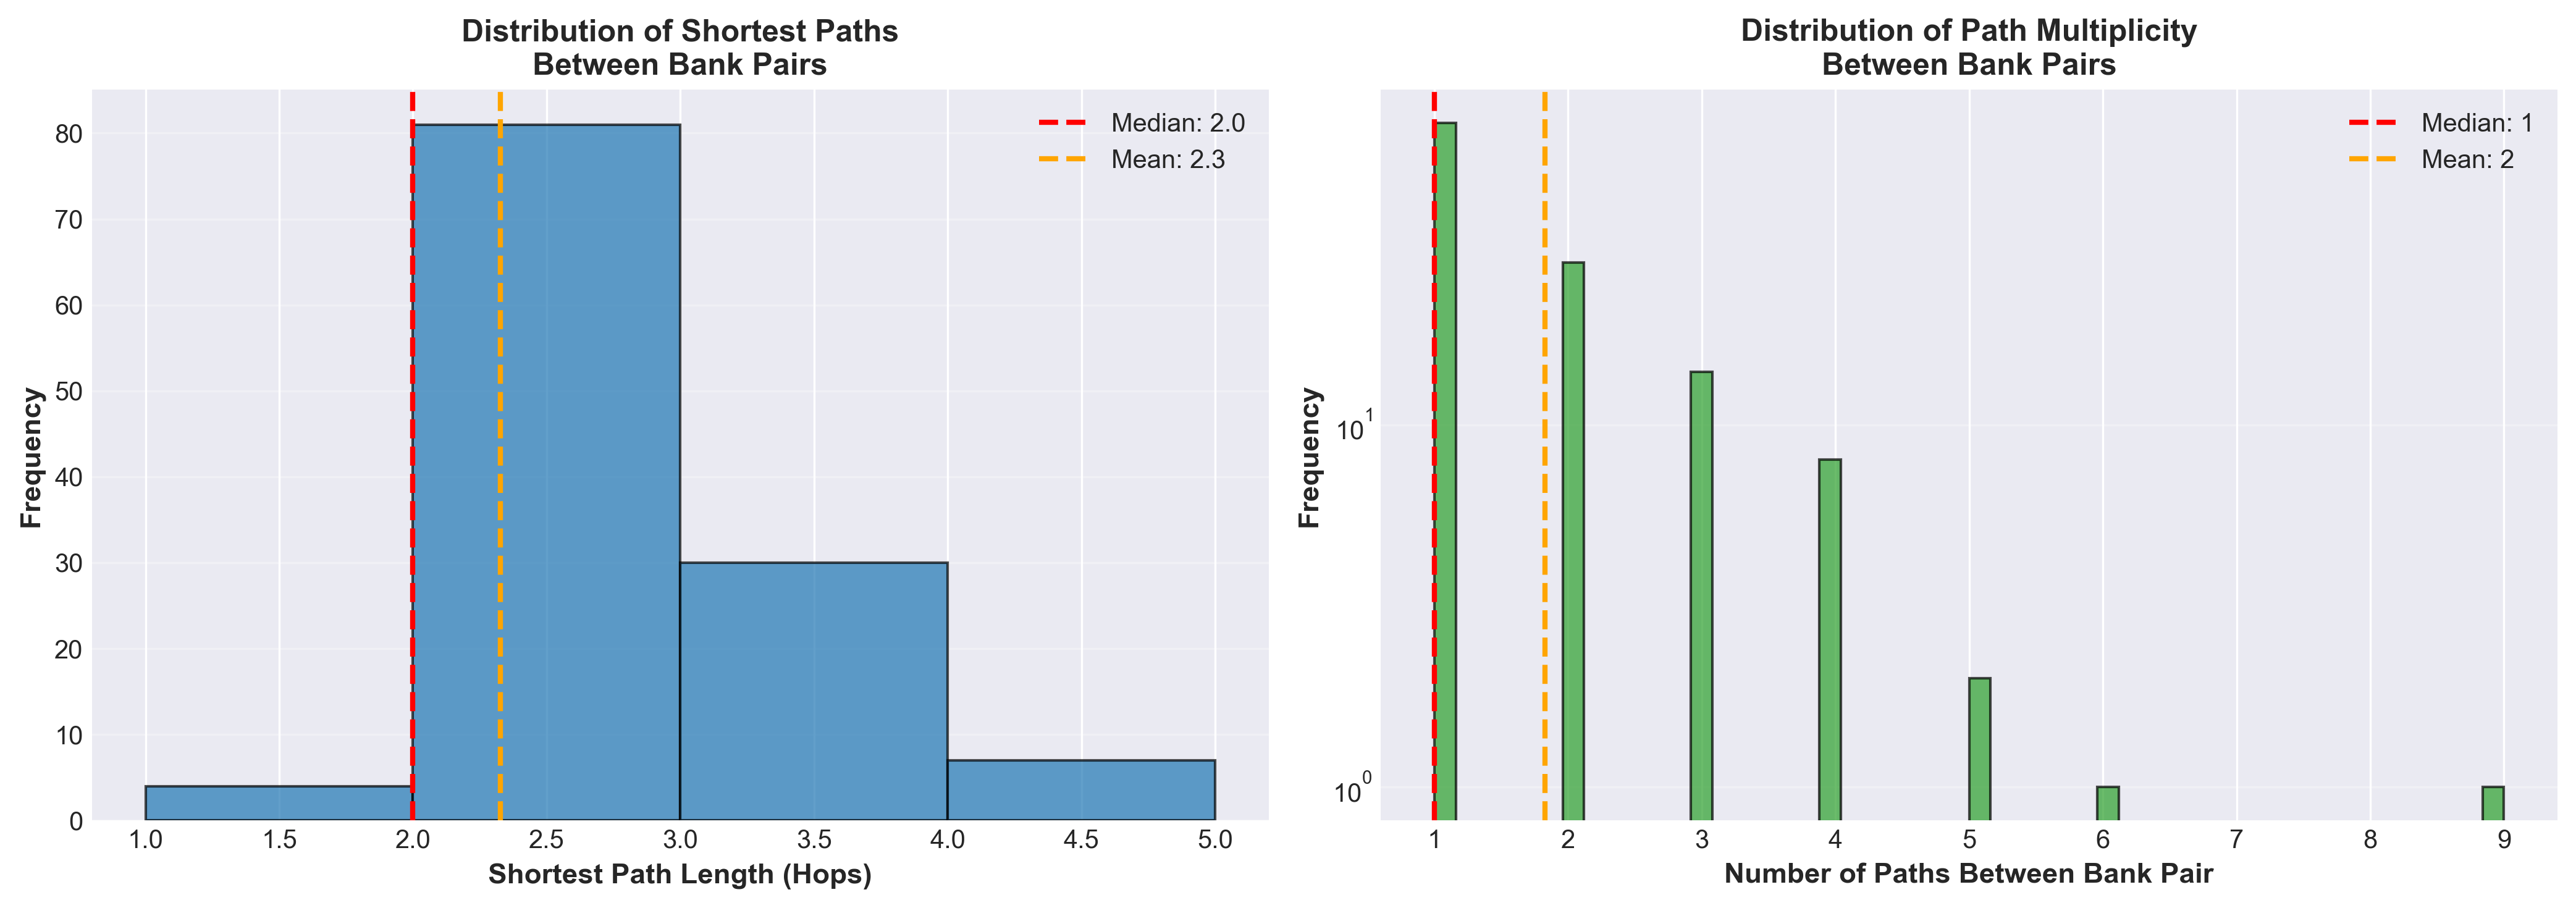
\includegraphics[width=\textwidth]{./figures/fig13_path_length_distribution.png}
\caption*{Figure 13. Path length and multiplicity distributions}
\end{figure}

Across all discovered bank pairs with at least one valid stress-propagation path:

\begin{table}[H]
\centering
\small
\begin{tabular}{l r}
\hline
Metric & Value \\
\hline
Total bank pairs with paths & 122 \\
Total unique paths & 223 \\
Average paths per pair & 1.83 \\
Minimum shortest path length & 1 hop \\
Maximum path length observed & 5 hops \\
Mean shortest path length & 2.33 hops \\
Median shortest path length & 2 hops \\
\hline
\end{tabular}
\end{table}

Path multiplicity is also concentrated at low values (median = 1), but with a right tail up to 9 paths for specific pairs. This indicates a dual structure: most bank pairs are connected through one dominant channel, while a smaller set has multiple alternate routes that can sustain contagion even if one channel weakens.

Overall, the results indicate that systemic vulnerability in this framework is driven by three interacting factors: (1) hub concentration among a few banks, (2) non-bank bridge intermediaries that connect otherwise distant bank pairs, and (3) short but redundant path structures among high-centrality nodes.

\section*{Discussion and Policy Implications}

### Academic Validation of Operational Feasibility

This framework constitutes real-world academic confirmation that publicly available data—Pillar 3 disclosures, MCA filings, CRISIL ratings, news feeds—can construct meaningful financial network topology without requiring privileged regulatory data. The IL&FS simulation demonstrates detection of elevated stress signals consistent with the timeline preceding default, suggesting operational early warning potential.

The contribution is methodological: demonstrating that knowledge graphs unify heterogeneous financial relationships (credit, shareholding, subsidiary chains) in a structure amenable to both visualization and algorithmic propagation. The entity selection approach—2,858 entities from 9,911 rated universe, capturing systemically significant exposures—provides a reproducible template for similar applications across emerging markets.

### Use Cases by Stakeholder

**Regulators (RBI/SEBI)**: The framework provides infrastructure for contagion scenario analysis. Rather than post-crisis forensics, regulators can use the network topology to trace how hypothetical stress at specific nodes would propagate through second-order connections. The fixed-point iteration algorithm makes contagion pathways explicit, enabling identification of systemically critical links.

**Bank Risk Teams**: ECL models under Ind AS 109 assess borrowers individually. They miss network effects: a borrower's other creditors' stress affects recovery probability. Our counterparty network maps reveal exposure concentrations that single-name limits overlook—multiple borrowers connected through common subsidiaries or sectors create correlated default risk invisible to traditional models.

**Institutional Investors**: Rating agencies maintained IL&FS at investment grade until crisis. Our hybrid stress scores—combining credit fundamentals with real-time sentiment—update continuously. When governance news turns negative, scores adjust without waiting for formal rating review. Independent signal for portfolio risk monitoring.

### Future Direction: Federated Learning for Sensitive Data

The framework currently operates on public disclosures. The next frontier involves sensitive credit data: internal bank loan books, real-time delinquency trends, covenant breach alerts. This data cannot leave bank networks due to regulatory and competitive constraints.

Federated learning offers a technically viable path forward. Under this architecture (McMahan et al., 2017; Yang et al., 2019), each participating bank runs the stress scoring model locally on its internal data within secure infrastructure. Only computed model updates or aggregated stress scores—not raw borrower-level data—propagate to a central coordinator for contagion modeling. The Secure Aggregation protocol (Bonawitz et al., 2017) ensures even the coordinator cannot reconstruct individual bank submissions.

Implementation would involve: (1) deploying containerized stress-scoring modules within each bank's secure compute environment; (2) using differential privacy mechanisms to add calibrated noise preventing membership inference; (3) aggregating bank-level stress contributions via weighted averaging aligned with exposure shares. The Flower framework (Beutel et al., 2020) or IBM FL provide production-ready orchestration for such deployments. European banking consortia have demonstrated this architecture for fraud detection; extending it to systemic risk monitoring represents natural evolution.

### Reference Point for Domain Applications

This framework can serve as blueprint for analogous applications: supply chain contagion mapping, healthcare network risk, or infrastructure grid vulnerabilities. The knowledge graph architecture is domain-agnostic; edge types and stress propagation rules adapt to context. When individual node health tells an incomplete story, network structure determines systemic resilience.

\section*{Limitations}

Several limitations define the boundaries of the present design. First, the graph depends heavily on public disclosures, which are uneven in quality, timing, and granularity. Second, not every contagion channel is observable: OTC derivatives, mutual fund holdings, and cross-border bilateral exposures are outside the current system. Third, the exposure layer remains incomplete for a large share of company nodes, so some rankings should be interpreted as partial but reliable slices rather than exhaustive counts. Finally, although the stress model is grounded in supervisory logic and graph theory, its parameters should still be refined through extended back-testing and historical case validation.

\section*{Conclusion}

This paper argues that systemic risk in India's credit sector is best understood as a network problem rather than an isolated balance-sheet problem. By merging disclosure-based entity resolution, stress scoring, sentiment analysis, and fixed-point contagion propagation into one knowledge graph, the proposed framework makes hidden dependencies visible and analytically useful.

The results are consistent with a system that is sparse overall yet highly exposed to hubs, bridge institutions, and short multi-hop contagion paths. That pattern helps explain why apparently localized distress can spread quickly once confidence weakens. For policymakers, banks, and investors, the practical implication is straightforward: better maps produce better early warnings. The framework offered here is not the final word on Indian systemic-risk measurement, but it is a credible and extensible starting point for doing that work with the data that are actually available.

\section*{References}

\aparef{Acharya, V. V., Pedersen, L. H., Philippon, T., \& Richardson, M. (2017). Measuring systemic risk. \textit{The Review of Financial Studies, 30}(1), 2--47.}

\aparef{Adrian, T., \& Brunnermeier, M. K. (2016). CoVaR. \textit{American Economic Review, 106}(7), 1705--1741.}

\aparef{Allen, F., \& Gale, D. (2000). Financial contagion. \textit{Journal of Political Economy, 108}(1), 1--33.}

\aparef{Araci, D. (2019). FinBERT: Financial sentiment analysis with pre-trained language models. \textit{arXiv}. \url{https://arxiv.org/abs/1908.10063}}

\aparef{Bajaj, R., \& Damodaran, A. (2023). Identification of domestic systemically important banks in India. \textit{Journal of Financial Stability, 65}, 101110.}

\aparef{Battiston, S., Puliga, M., Kaushik, R., Tasca, P., \& Caldarelli, G. (2012). DebtRank: Too central to fail? Financial networks, the FED and systemic risk. \textit{Scientific Reports, 2}, Article 541. \url{https://doi.org/10.1038/srep00541}}

\aparef{Brownlees, C., \& Engle, R. F. (2017). SRISK: A conditional capital shortfall measure of systemic risk. \textit{The Review of Financial Studies, 30}(1), 48--79.}

\aparef{Caccioli, F., Barucca, P., \& Kobayashi, T. (2018). Network models of financial systemic risk: A review. \textit{Journal of Computational Social Science, 1}(1), 81--114.}

\aparef{Chen, R.-R., \& Zhang, X. (2024). From liquidity risk to systemic risk: A use of knowledge graph. \textit{Journal of Financial Stability, 70}, 101195. \url{https://doi.org/10.1016/j.jfs.2023.101195}}

\aparef{CRISIL Ratings. (n.d.). \textit{Ratings and research}. \url{https://www.crisilratings.com/}}

\aparef{Grant Thornton. (2019). \textit{Forensic audit report of IL\&FS group}.}

\aparef{McMahan, H. B., Moore, E., Ramage, D., Hampson, S., \& Arcas, B. A. y. (2017). Communication-efficient learning of deep networks from decentralized data. In \textit{Proceedings of the 20th International Conference on Artificial Intelligence and Statistics} (pp.\ 1273--1282).}

\aparef{Ministry of Corporate Affairs. (2018). \textit{Order under Section 241 of the Companies Act, 2013 regarding IL\&FS Ltd.} Government of India.}

\aparef{NSE India. (2018). \textit{Market activity report: September-December 2018}.}

\aparef{NSE India. (n.d.-a). \textit{Corporate filings: Shareholding pattern}. \url{https://www.nseindia.com/companies-listing/corporate-filings-shareholding-pattern}}

\aparef{NSE India. (n.d.-b). \textit{Corporate integrated filing}. \url{https://www.nseindia.com/companies-listing/corporate-integrated-filing?integratedType=integratedfilingfinancials}}

\aparef{Open Government Data Platform India. (n.d.). \textit{Registrars of companies wise company master data}. \url{https://www.data.gov.in/resource/registrars-companies-roc-wise-company-master-data}}

\aparef{Press Information Bureau. (2025, February 24). \textit{Banking sector growth statistics FY2014-2024}. Ministry of Finance, Government of India. \url{https://www.pib.gov.in/PressReleasePage.aspx?PRID=2201357}}

\aparef{Reserve Bank of India. (2014). \textit{Master direction on Central Repository of Information on Large Credits (CRILC)}.}

\aparef{Reserve Bank of India. (2018). \textit{Financial stability report, December 2018}.}

\aparef{Reserve Bank of India. (2024). \textit{Report on trend and progress of banking in India 2023-24}.}

\aparef{Reserve Bank of India. (2025). \textit{Financial stability report, June 2025}.}

\aparef{Reserve Bank of India. (n.d.-a). \textit{Database on Indian economy: Statistical tables relating to banks in India}. \url{https://data.rbi.org.in/DBIE/\#/dbie/reports/Publication/Time-Series\%20Publications/Statistical\%20Tables\%20Relating\%20to\%20Banks\%20in\%20India/Tables\%20based\%20on\%20Annual\%20Accounts}}

\aparef{Reserve Bank of India. (n.d.-b). \textit{Revised prompt corrective action (PCA) framework for banks}. \url{https://www.rbi.org.in/Scripts/NotificationUser.aspx?Id=11131}}

\aparef{Reuters. (2018, October 1). India's IL\&FS crisis: A Lehman moment for country's shadow banks. \textit{Reuters}.}

\aparef{Serious Fraud Investigation Office. (2019). \textit{Interim report on IL\&FS group investigation}. Ministry of Corporate Affairs, Government of India.}

\aparef{Stander, Y. S. (2024). A news sentiment index to inform International Financial Reporting Standard 9 impairments. \textit{Journal of Risk and Financial Management, 17}(7), 282. \url{https://doi.org/10.3390/jrfm17070282}}

\aparef{Yang, Q., Liu, Y., Chen, T., \& Tong, Y. (2019). Federated machine learning: Concept and applications. \textit{ACM Transactions on Intelligent Systems and Technology, 10}(2), 1--19. \url{https://doi.org/10.1145/3298981}}

\end{document}
